\documentclass[11pt]{article}
\usepackage[margin=1in]{geometry}
\usepackage{volfit_preamble}
\graphicspath{{figures/}}

\title{\textbf{Observation Kalman Filtering}\\[2pt]
\large Denoising observed smiles without confusing noise with gaps\\[2pt]
\normalsize Vol-Fitter Technical Notes, No.~15}
\author{Vol-Fitter}
\date{\today}

% Note-local notation.
\newcommand{\obs}{\mathrm{obs}}
\newcommand{\gap}{\mathrm{gap}}
\newcommand{\calL}{\mathcal L}
\newcommand{\calI}{\mathcal I}
\newcommand{\calH}{\mathcal H}

\begin{document}
\maketitle

% Generated numbers (figures/gen_kalman.py). The fallback lets the note
% compile before the generator has run; values are then the last recorded
% backtest numbers (backend/backtest/FINDINGS_observation_filter.md).
\IfFileExists{figures/kalman_tables.tex}{%
% Auto-generated by gen_kalman.py — do not edit.
\newcommand{\KalGainLevel}{0.80}
\newcommand{\KalGainSkew}{0.72}
\newcommand{\KalGainCurv}{0.027}
\newcommand{\KalPostLevel}{20.32}
\newcommand{\KalPostSkew}{-0.364}
\newcommand{\KalPostCurv}{0.112}
\newcommand{\KalZstdSpikeTen}{5.16}
\newcommand{\KalZstdSpikeThirty}{1.75}
\newcommand{\KalErrPostSpike}{10.5}
\newcommand{\KalErrMeasSpike}{6.7}
\newcommand{\KalErrPredSpike}{47}
\newcommand{\KalWinSpike}{0.38}
\newcommand{\KalContraJacSpike}{15.8}
\newcommand{\KalContraFacSpike}{45.9}
\newcommand{\KalShockJacSpike}{38.6}
\newcommand{\KalShockFacSpike}{18.7}
\newcommand{\KalZstdHighTen}{1.43}
\newcommand{\KalZstdHighThirty}{0.82}
\newcommand{\KalErrPostHigh}{9.2}
\newcommand{\KalErrMeasHigh}{7.7}
\newcommand{\KalErrPredHigh}{31}
\newcommand{\KalWinHigh}{0.49}
\newcommand{\KalContraJacHigh}{10.5}
\newcommand{\KalContraFacHigh}{29.7}
\newcommand{\KalShockJacHigh}{78.6}
\newcommand{\KalShockFacHigh}{20.2}
\newcommand{\KalZstdLowTen}{1.32}
\newcommand{\KalZstdLowThirty}{1.05}
\newcommand{\KalErrPostLow}{5.3}
\newcommand{\KalErrMeasLow}{4.0}
\newcommand{\KalErrPredLow}{22}
\newcommand{\KalWinLow}{0.49}
\newcommand{\KalContraJacLow}{6.3}
\newcommand{\KalContraFacLow}{21.7}
\newcommand{\KalShockJacLow}{11.6}
\newcommand{\KalShockFacLow}{11.9}
\newcommand{\KalStepsTotal}{38\,181}
\newcommand{\KalShockImproveMin}{3}
\newcommand{\KalShockImproveMax}{7}
\newcommand{\KalActThinSpike}{6.5}
\newcommand{\KalActContraSpike}{9.1}
\newcommand{\KalActShockSpike}{19.5}
\newcommand{\KalOvlContraSpike}{12.1}
\newcommand{\KalRawContraSpike}{7.9}
\newcommand{\KalOvlShockSpike}{4.6}
\newcommand{\KalActThinHigh}{4.8}
\newcommand{\KalActContraHigh}{5.6}
\newcommand{\KalActShockHigh}{25.2}
\newcommand{\KalOvlContraHigh}{10.6}
\newcommand{\KalRawContraHigh}{9.8}
\newcommand{\KalOvlShockHigh}{7.9}
\newcommand{\KalActThinLow}{3.4}
\newcommand{\KalActContraLow}{4.5}
\newcommand{\KalActShockLow}{6.4}
\newcommand{\KalOvlContraLow}{6.3}
\newcommand{\KalRawContraLow}{5.4}
\newcommand{\KalOvlShockLow}{4.9}
\newcommand{\KalStepsVTwo}{39\,190}
\newcommand{\KalActZetaMin}{0.4}
\newcommand{\KalActZetaMax}{1.4}
\newcommand{\KalRefAgreement}{0}
\newcommand{\KalBlowupMinPts}{3}
\newcommand{\KalBlowupMaxPts}{28}
\newcommand{\KalEEMPost}{4.5}
\newcommand{\KalEEMMeas}{8.1}
\newcommand{\KalEEMZeta}{0.14}
\newcommand{\KalEFAZeta}{0.26}
}{%
\newcommand{\KalGainLevel}{0.80}%
\newcommand{\KalGainSkew}{0.72}%
\newcommand{\KalGainCurv}{0.027}%
\newcommand{\KalPostLevel}{20.32}%
\newcommand{\KalPostSkew}{-0.364}%
\newcommand{\KalPostCurv}{0.112}%
\newcommand{\KalZstdSpikeTen}{5.16}%
\newcommand{\KalZstdSpikeThirty}{1.76}%
\newcommand{\KalErrPostSpike}{10.5}%
\newcommand{\KalErrMeasSpike}{6.7}%
\newcommand{\KalErrPredSpike}{47}%
\newcommand{\KalWinSpike}{0.38}%
\newcommand{\KalContraJacSpike}{15.8}%
\newcommand{\KalContraFacSpike}{45.9}%
\newcommand{\KalZstdHighTen}{1.43}%
\newcommand{\KalZstdHighThirty}{0.82}%
\newcommand{\KalErrPostHigh}{9.2}%
\newcommand{\KalErrMeasHigh}{7.7}%
\newcommand{\KalErrPredHigh}{31}%
\newcommand{\KalWinHigh}{0.49}%
\newcommand{\KalContraJacHigh}{10.5}%
\newcommand{\KalContraFacHigh}{29.7}%
\newcommand{\KalZstdLowTen}{1.32}%
\newcommand{\KalZstdLowThirty}{1.05}%
\newcommand{\KalErrPostLow}{5.3}%
\newcommand{\KalErrMeasLow}{4.0}%
\newcommand{\KalErrPredLow}{22}%
\newcommand{\KalWinLow}{0.49}%
\newcommand{\KalContraJacLow}{6.3}%
\newcommand{\KalContraFacLow}{21.7}%
\newcommand{\KalStepsTotal}{38\,181}%
\newcommand{\KalShockJacSpike}{38.6}%
\newcommand{\KalShockFacSpike}{18.7}%
\newcommand{\KalShockJacHigh}{78.6}%
\newcommand{\KalShockJacLow}{11.6}%
\newcommand{\KalShockImproveMin}{3}%
\newcommand{\KalShockImproveMax}{8}%
\newcommand{\KalStepsVTwo}{39\,190}%
\newcommand{\KalActThinSpike}{6.5}%
\newcommand{\KalActThinHigh}{4.8}%
\newcommand{\KalActThinLow}{3.4}%
\newcommand{\KalActContraSpike}{9.1}%
\newcommand{\KalActContraHigh}{5.6}%
\newcommand{\KalActContraLow}{4.5}%
\newcommand{\KalActShockSpike}{19.5}%
\newcommand{\KalActShockHigh}{25.2}%
\newcommand{\KalOvlContraSpike}{12.1}%
\newcommand{\KalOvlContraHigh}{10.6}%
\newcommand{\KalOvlContraLow}{6.3}%
\newcommand{\KalRawContraSpike}{7.9}%
\newcommand{\KalRawContraHigh}{9.8}%
\newcommand{\KalRawContraLow}{5.4}%
\newcommand{\KalOvlShockSpike}{4.6}%
\newcommand{\KalOvlShockHigh}{7.9}%
\newcommand{\KalOvlShockLow}{4.9}%
\newcommand{\KalActZetaMin}{0.4}%
\newcommand{\KalActZetaMax}{1.4}%
\newcommand{\KalRefAgreement}{10^{-16}}%
\newcommand{\KalBlowupMinPts}{3}%
\newcommand{\KalBlowupMaxPts}{28}%
\newcommand{\KalEEMPost}{4.5}%
\newcommand{\KalEEMMeas}{8.1}%
\newcommand{\KalEEMZeta}{0.14}%
\newcommand{\KalEFAZeta}{0.26}%
}

\begin{abstract}
Prior persistence and Kalman filtering both pull a smile away from a raw,
current-market fit, so they are easy to confuse in implementation. They must
not be confused mathematically. Prior persistence (Note~13) is a \emph{gap
regularizer}: it keeps unobserved or weakly identified smile functionals near
a transported prior and turns itself off where today's quotes already identify
the functional. The observation filter of this note is a \emph{temporal state
estimator}: it assumes the current smile is observed through noisy, sometimes
contradictory quotes, predicts the smile from the previous filtered state
under the SSR transport of Note~12, and updates according to the relative
precision of prediction and observation. The state is not raw option mids but
the compact arbitrage-safe ATM handles of Note~01; the measurement covariance
is propagated from the data-only fit's solution Jacobian through the handle
map, inflated by realized inconsistency; and active mode is a one-stage MAP
calibration so the same quotes are never counted twice. The machinery is in
production, and the note now reports what it measured. In the canonical case
file a stale-strike curvature kink is accepted at gain \KalGainCurv\ while the
genuine level move passes at gain \KalGainLevel. A \KalStepsTotal-step
temporal backtest over three market regimes flipped the clock process noise
from the design value of $10$ to $30$ vol bp per $\sqrt{\text{day}}$
(standardized residuals collapse toward $1$ in every regime, shock lag shrinks
\KalShockImproveMin--\KalShockImproveMax$\times$), confirmed the
Jacobian-propagated covariance as the default route ($2$--$3\times$ better
contradiction rejection than the factor route in every regime), and taught the
one genuinely structural lesson: on coarse-strike chains the full-covariance
update let a junk curvature innovation drag the ATM level through off-diagonal
gains, so production runs the update per handle. A second,
\KalStepsVTwo-step sweep with the adaptive clock on then scored active mode
itself: the one-stage MAP is the best denoiser wherever denoising is the job
--- on high-vol contradiction days \KalActContraHigh\ vs \KalRawContraHigh\ bp
for the raw fit it consumes --- and its one measured weakness, shock lag
(the adaptive clock is overlay-only), is the flagged item before any
active-by-default.
\end{abstract}

\tableofcontents
\newpage

%======================================================================
\section{The production symptom}
\label{sec:symptom}

A sparse wing and a noisy cluster are different failures.

In a sparse wing, the desk has almost no market information. A data-only fit
can extend the ATM skew into the tail and create a new signal where no option
actually traded. Note~13 solved that problem with an activation gate: the
prior is strong in the gap and exactly off where the data is sufficient.

In a noisy cluster, the desk has information, but it is internally
inconsistent. Two adjacent strikes may imply a local kink because one market
is stale, a wide bid--ask band may make the mid meaningless, or an American
wing repair (Note~05) may have preserved spread while lowering the reliable
rank of the wing. The right answer is not ``fill with yesterday''; the right
answer is ``infer the latent current smile under observation noise.''

\begin{invariant}
\begin{enumerate}[leftmargin=1.6em]
\item Prior persistence acts only on functionals not identified by the current
market at the required precision.
\item Observation filtering acts only through an explicit prediction
covariance and an explicit measurement covariance.
\item The same quote cannot be used once to create a filtered posterior and
then again as an independent calibration datum (\cref{prop:nodouble}).
\item The filter state is an arbitrage-safe coordinate --- the exact ATM
handles of Note~01 --- never a free raw-IV curve and never native local-vol
parameters.
\item Every filtered output reports prediction, observation, innovation, gain
and posterior uncertainty.
\end{enumerate}
\end{invariant}

The two features therefore answer two different questions:
\[
\begin{array}{ll}
\text{Prior persistence:} & \text{Where do we lack enough observations to
identify the smile?}\\[2pt]
\text{Kalman filtering:} & \text{Given observations here, how noisy are they?}
\end{array}
\]
The implementation preserves that distinction all the way to the UI, and the
temporal backtest of \cref{sec:backtest} scores it: the success criterion is
lower held-out error on \emph{noisy} snapshots with no meaningful lag on
high-quality moves --- explicitly not ``lower every RMS''.

%======================================================================
\section{Two regularizers, two measures}
\label{sec:split}

Let $x_t\in\R^d$ denote the latent smile state of one node at snapshot time
$t$: in production this is the compact handle vector
\[
x_t=(\sigma_{\atm,t},\,s_{\atm,t},\,\kappa_{\atm,t})\T,
\]
the same three coordinates the graph extrapolator of Note~14 propagates
(signed operators such as RR25, BF25 and var-swap are a dimension-agnostic
extension left for after the pilot). Let $q_t$ be the prepared quote set after
forwards, de-Americanization, event-clock conversion, bid--ask band
construction and quote edits.

\subsection{Prior persistence}

Prior persistence is a penalty in a calibration objective. With a prior state
$x_t^0$ transported to the current forward, and functionals
$O_j:\R^d\to\R$, Note~13 has the universal form
\begin{equation}
\calL_{\mathrm{persist}}(x)
=\half\sum_j
\lambda_j^{\gap}
\left(\frac{O_j(x)-O_j(x_t^0)}{a_j}\right)^2,
\qquad
\lambda_j^{\gap}
=\lambda_j^0
\max\!\left(1-\frac{\pi^{\obs}_j}{\pi^{\mathrm{req}}_j},0\right)^\gamma .
\label{eq:persistence}
\end{equation}
The gate is driven by \emph{identifiability}: when current quotes identify
functional $O_j$ at or above the required precision, $\lambda_j^{\gap}=0$.
Thus prior persistence is not primarily a denoiser. It is a rule for refusing
to invent signal outside the support of the observation.

\subsection{Observation filtering}

A Kalman filter is instead a sequential estimator. It starts from the previous
posterior law for $x_{t-1}$, transports it forward, then combines the
transported prediction with today's noisy observation. In the linear-Gaussian
handle model,
\begin{align}
x_t &= \Phi_t x_{t-1}+u_t+\eta_t,
&\eta_t&\sim\mathcal N(0,Q_t), \label{eq:state}\\
z_t &= H_t x_t+\epsilon_t,
&\epsilon_t&\sim\mathcal N(0,R_t), \label{eq:measurement}
\end{align}
where $z_t$ is not a raw quote vector; it is a noisy handle estimate extracted
from today's prepared quotes. $Q_t$ is process covariance: time elapsed, spot
move, event risk and transport distance. $R_t$ is measurement covariance:
bid--ask width, quote density, stale fields, de-Americanization repairs, band
slack and contradictory close strikes.

\begin{heuristic}
Persistence says ``do not put signal where the market did not speak.''
Filtering says ``when the market speaks with a noisy voice, infer what it
probably meant.'' Both can pull toward a previous surface, but the sufficient
statistic is different: persistence uses a \emph{gap}; filtering uses a
\emph{covariance}.
\end{heuristic}

%======================================================================
\section{The Kalman object}
\label{sec:kalman}

The Vol-Fitter implements the filter in covariance form, matching the graph
posterior style of Note~14. For a direct handle observation $H_t=I$ the form
is especially transparent, but the equations allow a subset or a linear
operator measurement.

\begin{definition}[Predicted and observed handle laws]
\label{def:laws}
At snapshot $t$, the prediction law and the measurement law are
\[
x_t\given\mathcal F_{t-1}\sim\mathcal N(m_t^-,P_t^-),
\qquad
z_t\given x_t\sim\mathcal N(H_t x_t,R_t).
\]
$m_t^-$ is the transported previous filtered state; $P_t^-$ is its transported
uncertainty plus process noise. $z_t$ and $R_t$ are extracted from today's
prepared quotes without using prior persistence.
\end{definition}

The central update is
\begin{equation}
\boxed{\;
\begin{aligned}
S_t&=H_tP_t^-H_t\T+R_t,\\
K_t&=P_t^-H_t\T S_t^{-1},\\
m_t^+&=m_t^-+K_t\big(z_t-H_tm_t^-\big),\\
P_t^+&=(I-K_tH_t)P_t^-(I-K_tH_t)\T+K_tR_tK_t\T .
\end{aligned}
\;}
\label{eq:kalman}
\end{equation}
The last line is the Joseph form; it is a little longer than
$P_t^+=(I-K_tH_t)P_t^-$, but it preserves symmetry and positive
semidefiniteness for \emph{any} gain --- which is precisely what makes the
pilot gain cap below safe: a capped $K$ is still a valid, merely suboptimal,
linear gain. The production body is small enough to quote whole:

\begin{lstlisting}[caption={The production update (quoted from
\texttt{volfit/calib/observation\_filter.py}): \cref{eq:kalman} with the
own-gain pilot cap, Joseph covariance, and an explicit PSD guard.},
label={lst:crux}]
innovation = z - H @ m
S = H @ P @ H.T + R
K = np.linalg.solve(S.T, (P @ H.T).T).T   # gain without an explicit inverse
if max_gain < 1.0:                        # pilot cap: scales OWN-gains only
    own = np.abs(np.diag(K @ H))
    scale = np.minimum(1.0, max_gain / np.maximum(own, 1e-300))
    K = K * scale[:, None]
out_mean = m + K @ innovation
i_kh = np.eye(m.size) - K @ H
out_cov = i_kh @ P @ i_kh.T + K @ R @ K.T # Joseph form: PSD for ANY gain
out_cov = 0.5 * (out_cov + out_cov.T)
if np.any(np.linalg.eigvalsh(out_cov) < -1e-12):
    raise FloatingPointError("posterior covariance lost PSD")
\end{lstlisting}

\begin{proposition}[Precision-weighted shrinkage]
\label{prop:scalar}
In one dimension with $H_t=1$, prediction variance $p$ and measurement
variance $r$, the posterior mean is
\[
m^+=\frac{r}{p+r}m^-+\frac{p}{p+r}z,
\]
and the Kalman gain is $K=p/(p+r)$.
\end{proposition}

\begin{proof}
The innovation variance is $S=p+r$, so $K=p/S$. Substituting in
$m^+=m^-+K(z-m^-)$ gives
$m^+=(1-K)m^-+Kz=r(p+r)^{-1}m^-+p(p+r)^{-1}z$.
\end{proof}

\Cref{prop:scalar} is the whole desk intuition. If today's observation is
tight ($r\ll p$), the filtered smile moves to the market. If today's
observation is noisy ($r\gg p$), it stays near the transported prediction. The
movement is not controlled by whether the region is observed; it is controlled
by the relative uncertainties of prediction and observation.

\begin{remark}[Production runs \cref{eq:kalman} per handle]
\label{rem:diagonal}
The design allowed a full $d\times d$ update. Production diagonalizes $P_t^-$
and $R_t$ before the update (\texttt{DIAGONAL\_UPDATE} in
\texttt{volfit/api/observation\_filter.py}), so each handle receives exactly
the scalar gain of \cref{prop:scalar} --- the same convention as the Note~14
graph posterior. That is a measured decision, not an aesthetic one: the
backtest showed the off-diagonal gains of the full update turning a junk
curvature innovation into a multi-vol-point ATM error on coarse-strike chains.
The second case file of \cref{sec:case} tells that incident in full; the
full-covariance update remains available for later study.
\end{remark}

%======================================================================
\section{Where the observation covariance comes from}
\label{sec:measurement}

The hard part is not the Kalman algebra. The hard part is building a
measurement covariance $R_t$ that reflects the quote set honestly. Production
has two routes, selected by \texttt{filterCovarianceMode}: the default
\emph{Jacobian route} propagates the fit's observed information through the
handle map, and the \emph{factor route} reuses the graph layer's precision
vocabulary as a fallback and A/B diagnostic. Both live in
\texttt{volfit/calib/observation\_measurement.py}.

\subsection{Do not filter raw mids}

Raw contracts are a poor state space. The OTM side changes when the forward
moves; contracts appear and disappear; American contracts need early-exercise
removal; a strike can be inside a wide spread but far from its midpoint; and a
raw implied-vol vector is not guaranteed to remain butterfly-free after
smoothing. The filter begins after the existing quote-prep pipeline in
\texttt{volfit/api/quotes.py}.

\subsection{Extract a noisy handle observation}

The observation extractor is a two-step map:
\begin{equation}
z_t=\calH\Big(\argmin_\theta\
\calL_{\mathrm{quote}}(\theta;q_t)+\calL_{\mathrm{intrinsic}}(\theta)\Big),
\label{eq:extract}
\end{equation}
where $\calL_{\mathrm{quote}}$ is the vega-normalized, bid--ask-aware loss of
Note~07, $\calL_{\mathrm{intrinsic}}$ contains only the intrinsic model
regularization needed for a valid no-arbitrage smile (never temporal prior
persistence), and $\calH$ reads the exact ATM handles off the fitted slice. In
production the carrier is the LQD backbone --- always fitted, model-agnostic,
with closed-form handles (Note~01) --- so
$z_t=(\hat\sigma_{\atm},\hat s_{\atm},\hat\kappa_{\atm})$ costs nothing extra.
When the committed fit did receive persistence targets (hybrid mode with an
active prior), the measurement is flagged \texttt{contaminated} rather than
silently trusted; Note~13's activation gate keeps the overlap near zero
exactly where the filter has signal, and the opt-in
\texttt{filterDataOnlyPrepass} buys a strictly clean $z_t$ at the cost of one
extra data-only fit per node.

\subsection{The Jacobian route (default)}
\label{sec:jacroute}

Near the optimum, linearize the residual stack as
$r(\theta)\approx r(\hat\theta)+J(\theta-\hat\theta)$. If the handle map is
$x=g(\theta)$ with Jacobian $G=\partial g/\partial\theta$, the
observed-information approximation is
\begin{equation}
\calI_\theta=J\T WJ+\Lambda_{\mathrm{intrinsic}},
\qquad
R_x\approx G\,\calI_\theta\pinv\, G\T .
\label{eq:cov-delta}
\end{equation}
Implementation makes this nearly free. Every parametric calibrator solves via
least squares and retains the solution Jacobian in a diagnostics side-channel;
the square-root weights and inverse-vega scaling are already folded into its
rows, so $J\T J$ \emph{is} the information in vol units, with the intrinsic
regularization rows (ridge, calendar, barrier) supplying
$\Lambda_{\mathrm{intrinsic}}$ automatically. $G$ is a central finite
difference of the handle map --- slice \emph{builds}, not fits, on the coarse
optimization grid. The pseudo-inverse in \cref{eq:cov-delta} is deliberately a
\emph{regularized} eigen-inverse: eigenvalues below
$\texttt{INFO\_RANK\_RTOL}\cdot\lambda_{\max}$ are clamped \emph{up} to the
cutoff, so a $\theta$-direction the quotes do not identify contributes a
large-but-finite handle variance. A strict pseudo-inverse would do the
opposite --- read an unidentified direction as \emph{zero} uncertainty --- which
is the one failure mode a filter must never inherit from its measurement.

The covariance is then inflated by realized inconsistency:
\begin{equation}
R_t=\rho_t R_x,\qquad
\rho_t=\operatorname{clip}\!\left(\frac{\chi_t^2}{\max(m-d,1)},\,1,\,
\rho_{\max}\right),
\qquad
\chi_t^2=r(\hat\theta)\T W r(\hat\theta),
\label{eq:resid-inflation}
\end{equation}
with $\chi^2$ read off the quote rows only and the cap $\rho_{\max}$
(\texttt{RESID\_INFLATION\_CAP}) preventing one broken chain from poisoning
the state. This is the mechanism that makes close-strike contradictions
visible to the filter: a contradictory cluster may have many quotes, but if it
cannot be fitted within its stated noise, $\rho_t$ grows and the Kalman gain
falls in the directions the cluster does not reliably identify.

\begin{remark}[Bands and covariance]
For bid--ask mode, quotes inside the band should not pretend to identify the
mid. On the Jacobian route this comes for free: inactive hinge rows
differentiate to zero inside the spread, so in-band quotes contribute nothing
to $J\T WJ$, and only the weak mid anchor remains at its small weight. This
matches Note~07's semantics --- inside the spread the market is a set, not a
point --- with no special-casing, a concrete advantage over the factor route,
which must proxy band width through a spread factor.
\end{remark}

\subsection{Units: information is only information in stated noise}
\label{sec:units}

\begin{caution}
The production quote weights are \emph{relative} (equal or time-value
density, Note~07), not $1/\text{noise}^2$. Read at face value, $J\T WJ$ is
therefore the observed information under an implied noise of one full
volatility point per quote --- so small that $R_x$ saturates the sanity
envelope and the filter freezes. The shipped builder fixes the units at the
source: the data rows of $J$ and $r$ are divided by the stated per-quote noise
standard deviation --- the bid--ask half-spread floored at
\texttt{RMS\_FLOOR}, or the haircut --- \emph{before} the information and
$\chi^2$ are formed, while the intrinsic regularization rows keep their own
scale (they are a prior, not a measurement). $R_t$ then obeys the quadratic
contract the algebra assumes: doubling the stated noise quadruples the
covariance. The same scale $s_q$ reappears twice in active mode
(\cref{sec:active}): the prediction prior enters the fit at weight
$\lambda_j=s_q^2/\Var(O_j)$, and the posterior information is recovered by
unwhitening \emph{all} rows by $s_q$ --- one consistent value in both places,
or the MAP algebra silently breaks.
\end{caution}

\subsection{The factor route (fallback and A/B column)}

The cheaper builder reuses the existing precision vocabulary,
\begin{equation}
R_t^{-1}
=\diag(c_h)\,
\pi_{\mathrm{fit}}\,
f_{\mathrm{density}}\,
f_{\mathrm{spread}}\,
f_{\mathrm{fresh}},
\label{eq:cheapR}
\end{equation}
where $c_h$ is per-handle confidence, $\pi_{\mathrm{fit}}$ is inverse squared
RMS with a floor and cap, and the scalar factors are exactly those of
\texttt{volfit/graph/precision.py}. The realized misfit already lives in the
RMS factor, so no separate $\rho$ inflation is applied (it would
double-count). This route survives as the fallback when no solution Jacobian
was retained (cached fits) and as the sweep's A/B diagnostic column --- which
is how the Jacobian route's advantage got \emph{measured} rather than assumed
(\cref{sec:backtest}).

%======================================================================
\section{The prediction law and the state's life cycle}
\label{sec:prediction}

\subsection{Transport and process noise}

The prediction must transport the previous filtered smile before comparing it
with today's quotes. For a handle state,
\begin{equation}
m_t^-=\mathcal T_t(m_{t-1}^+),
\qquad
P_t^-=A_tP_{t-1}^+A_t\T+Q_t,
\label{eq:transport}
\end{equation}
where $\mathcal T_t$ is the SSR/spot-vol transport of Note~12. Production uses
the first-order handle map for a log-forward move $h$,
\begin{equation}
\sigma_{\atm}'=\sigma_{\atm}+\mathrm{SSR}\cdot s_{\atm}\,h,
\qquad
s_{\atm}'=s_{\atm}+\kappa_{\atm}\,h,
\qquad
\kappa_{\atm}'=\kappa_{\atm},
\label{eq:transport-handles}
\end{equation}
with $A_t=I$ (the uncertainty growth is carried entirely by $Q_t$; a full
curve transport is not available for a bare handle vector, and seeding uses
the exact curve transport through the prior machinery instead). The process
covariance is a diagonal sum,
\begin{equation}
Q_t=Q_{\mathrm{clock}}(\Delta t)+Q_{\mathrm{spot}}(\abs h)
+Q_{\mathrm{event}}+Q_{\mathrm{source}}+Q_{\mathrm{model}},
\label{eq:Q}
\end{equation}
with the following meanings:
\begin{description}[leftmargin=1.7em,style=nextline]
\item[Clock noise.]
Volatility surfaces diffuse through time; the baseline is
$q_h^2\,\Delta t$ per handle (std $=q_h\sqrt{\Delta t}$). The ATM scale $q$ is
the headline knob \texttt{filterProcessVolBpSqrtDay}: the design note proposed
$10$ vol bp$/\sqrt{\text{day}}$, and the three-regime backtest flipped the
shipped default to $30$ (\cref{sec:backtest}).
\item[Spot transport noise.]
The larger the log-forward move $h=\log(F_t/F_{t-1})$, the less certain the
transported state: std $=\texttt{filterTransportNoiseScale}\cdot\abs h$ in
each handle's typical move scale. This is the same intuition as the
transport-distance factor in prior persistence.
\item[Event noise.]
Known event windows widen the prediction before the event resolves. The event
clock of the calibration changes the time variable; this term admits that the
shape response itself is uncertain.
\item[Source noise.]
Switching provider, as-of mode, or live/previous-close source widens or resets
the filter. A live quote stream and a prior-close snapshot are not the same
stochastic clock.
\item[Model noise.]
If the display model changes, the filtered handle state may persist (it is
model-agnostic), but model-specific parameters do not.
\end{description}

\begin{caution}
Do not filter native local-vol parameters. The local-vol grid (Note~04) is a
projection machinery with its own PDE stability and no-arbitrage constraints.
Filter the target smile handles, then project or refit the local-vol surface
to that target.
\end{caution}

\subsection{Seeding, resets, and what survives a recalibration}
\label{sec:lifecycle}

A filter is only as trustworthy as its life-cycle rules, so production pins
them down explicitly (\texttt{volfit/api/observation\_filter.py}):

\begin{description}[leftmargin=1.7em,style=nextline]
\item[Seeding.] When a saved prior snapshot exists, the first state is the
\emph{transported} prior through the provenance hierarchy of Note~13, with
covariance from the provenance-tier precisions. When none exists, the seed is
the committed fit's \emph{own} backbone handles at bootstrap-tier precision
--- the same information a bootstrap fetch would produce, for free. There is
deliberately no hidden extra fit on the seeding path (\cref{app:perf} records
the incident that made this a rule).
\item[Resets.] A manual quote edit moves the session version and resets the
node (the edited chain invalidates the measurement the state was built on); a
calendar gap beyond \texttt{filterResetHours} resets as \texttt{stale}
(predicting across a long dark period is worse than reseeding from the
transported prior); a source or as-of change wipes the store outright (the
strict source-reset policy). Every reset records its reason in the
diagnostics payload.
\item[Recalibration keeps the state.] The update is sequential --- one step per
genuinely \emph{new} observation, idempotent per (node, data version, session
version). Recalibrating an unchanged snapshot re-reads the stored state; a
refetch is a new observation, not a reset.
\end{description}

%======================================================================
\section{The clean architecture}
\label{sec:architecture}

There are two mathematically safe ways to let the filter act, and production
ships both behind \texttt{observationFilterMode}
(\texttt{volfit/api/filter\_mode.py}): \texttt{off} is byte-identical to the
filter never existing, \texttt{overlay} computes and displays, \texttt{active}
steers calibration as a one-stage MAP.

\subsection{Overlay mode: compute, display, do not affect calibration}

Overlay mode is the pilot delivery. On every committed fit the app layer
prepares quotes, extracts $(z_t,R_t)$ from the data-only information, predicts
$(m_t^-,P_t^-)$ from the previous state, applies \cref{eq:kalman} per handle,
and stores the full audit trail --- prediction, observation, innovation, gain,
posterior --- for the smile viewer, which draws the raw calibration, the
transported prediction and the filtered curve with its credible band. This
mode cannot double-count quotes because the posterior never feeds back into
the fit; it is therefore the sandbox in which $Q_t$, $R_t$ and the reset rules
were tuned (\cref{sec:backtest}).

\subsection{Active mode: one-stage MAP, not posterior plus quotes}
\label{sec:active}

Active mode must not first build $m_t^+$ from today's quotes and then add
$m_t^+$ as a prior while fitting the same quotes again. That counts $q_t$
twice. The correct active objective is the one-step MAP problem
\begin{equation}
\calL_{\mathrm{active}}(\theta)
=\calL_{\mathrm{quote}}(\theta;q_t)
+\half\norm[\big]{\calH(\theta)-m_t^-}_{(P_t^-)^{-1}}^2
+\calL_{\mathrm{intrinsic}}(\theta)
+\calL_{\mathrm{persist},\perp}(\theta).
\label{eq:active-map}
\end{equation}
Here $\calH(\theta)$ extracts the filtered handle coordinates from the model,
the second term is the Kalman prediction prior, and the quote likelihood is
today's market. In the linear-Gaussian case, minimizing \cref{eq:active-map}
gives the same $m_t^+$ as \cref{eq:kalman}; in the nonlinear smile case it is
the extended-Kalman/MAP version.

\begin{proposition}[No double counting in the MAP form]
\label{prop:nodouble}
If the model is linear, the quote extractor is $z=H x+\epsilon$ with
$\epsilon\sim\mathcal N(0,R)$, and the prediction is
$x\sim\mathcal N(m^-,P^-)$, then the minimizer of
\[
\half\norm{z-Hx}_{R^{-1}}^2+\half\norm{x-m^-}_{(P^-)^{-1}}^2
\]
is the Kalman posterior mean in \cref{eq:kalman}.
\end{proposition}

\begin{proof}
The first-order condition is
\[
\big(H\T R^{-1}H+(P^-)^{-1}\big)x
=H\T R^{-1}z+(P^-)^{-1}m^- .
\]
The Woodbury identity rewrites the inverse of the left-hand side as
$P^- - P^-H\T(HP^-H\T+R)^{-1}HP^-$. Substitution gives
$x=m^-+P^-H\T(HP^-H\T+R)^{-1}(z-Hm^-)$, which is \cref{eq:kalman}.
\end{proof}

Production realizes \cref{eq:active-map} with four locked decisions
(\texttt{build\_filter\_prior} in
\texttt{volfit/calib/observation\_filter.py}; the MAP bookkeeping in
\texttt{volfit/api/observation\_filter.py}):

\begin{enumerate}[leftmargin=1.6em]
\item \textbf{The prediction prior is an \emph{ungated} operator target.} It
reuses the smile-factor stencil legs at $k\in\{-h,0,h\}$ with
$h=\texttt{FILTER\_STENCIL\_H}=0.06$: on a locally quadratic smile the stencil
identities
$\sigma(h)-\sigma(-h)=2h\,s_{\atm}$ and
$\sigma(h)-2\sigma(0)+\sigma(-h)=h^2\kappa_{\atm}$
are \emph{exact}, so the handle targets convert to stencil targets with no
approximation beyond local quadraticity. Because these are ordinary operator
residuals, the prior flows to LQD, SVI and Multi-Core Sigmoid (MCS) through
the existing plumbing with zero per-model wiring --- and, crucially, it
carries \emph{no} activation gate. The Kalman prior is always on at its covariance weight; that
is precisely the persistence/filter distinction of \cref{sec:split}.
\item \textbf{The weights are the MAP objective in the fit's own units.} The
quote rows are (near-)unit-weighted vol errors, i.e.\ the true MAP objective
$\sum_i(e_i/s_q)^2+\sum_j d_j^2/P^-_{jj}$ multiplied through by $s_q^2$, so
the consistent prior weight is $\lambda_j=s_q^2/\Var(O_j)$ with $s_q$ the
node's typical stated per-quote noise (the median bid--ask half-spread,
floored --- the same $s_q$ as \cref{sec:units}).
\item \textbf{Persistence auto-exclusion is hard-coded.} When the mode is
\texttt{active}, \texttt{resolve\_prior\_mode}
(\texttt{volfit/api/prior\_mode.py}) drops every persistence builder
overlapping the handle coordinates --- operators, smile factors, the near-ATM
strike anchor. What survives is exactly what the filter state does not carry:
the deep-tail strike anchor and the graph's dark-node baseline. There is
deliberately no knob; two anchors to the same previous state would violate
invariant 3.
\item \textbf{No second update.} The committed fit \emph{is} the one-stage MAP
solution, so $m^+$ is simply its backbone handles, and $P^+$ comes from
unwhitening the full solver information (data rows plus whitened prior rows)
by the same $s_q$ --- landing exactly at
$\calI_{\mathrm{data}}+(P^-)^{-1}$, the posterior information of
\cref{prop:nodouble}. Applying \cref{eq:kalman} again against the same quotes
would double-count them; the test suite locks the MAP-equals-Kalman identity
to $10^{-10}$. One guard is added on top: $P^+$ is capped at $P^-$ per handle,
because information only adds --- inconsistent data ($\rho>1$) should drive
$P^+$ \emph{toward} the prediction uncertainty, never beyond it.
\end{enumerate}

\subsection{Where prior persistence remains}

Prior persistence remains available in active mode, with explicit semantics:
it acts on deep tails and operator baskets not represented in the Kalman
state; it provides the saved prior from which the first filtered state is
seeded; and it acts on dark graph nodes that have no current quote
observation. It does not also anchor ATM/skew/curvature to the same previous
state that already appears as $m_t^-$ in the Kalman term --- the auto-exclusion
above makes this structural rather than procedural.

%======================================================================
\section{Two case files}
\label{sec:case}

The first case file is the note's original design vignette, now computed by
the production update (\texttt{gen\_kalman.py} feeds the numbers below through
\texttt{kalman\_update}; \cref{fig:case}). The second is a real incident from
the temporal backtest --- the one that changed the production update.

\begin{example}[title={Case file: close-strike contradiction versus true gap}]
\textbf{Setup.} A one-month equity smile has nine near-ATM quotes and no
reliable quotes beyond $25\Delta$. The previous filtered state transported to
today is
\[
m^-=(20.0\%,\ -0.35,\ 0.10),\qquad
\sqrt{\diag P^-}=(0.30\%,\ 0.08,\ 0.05).
\]
The near-ATM quotes imply a data-only handle observation
\[
z=(20.4\%,\ -0.37,\ 0.55).
\]
The ATM level and skew are consistent, but one stale close strike forces a
very large curvature if the fit chases mids literally.

\textbf{Diagnosis.} Quote density alone would say the region is well observed.
Therefore prior persistence must switch off for ATM/skew/curvature; using it
to pull curvature back would violate the Note~13 rule. The contradiction
instead appears as measurement noise, through the $\chi^2$ inflation of
\cref{eq:resid-inflation}: the observation standard deviations come out as
\[
\sqrt{\diag R}=(0.15\%,\ 0.05,\ 0.30).
\]
The production per-handle gains are
\[
K_{\sigma}=\KalGainLevel,\qquad
K_s=\KalGainSkew,\qquad
K_\kappa=\KalGainCurv.
\]

\textbf{Filter.} The update moves the real observed level and skew,
$m^+_\sigma=\KalPostLevel\%$ and $m^+_s=\KalPostSkew$, but barely accepts the
isolated curvature kink: $m^+_\kappa=\KalPostCurv$.

\textbf{Persistence.} The unquoted wing is a different matter. For a deep-tail
functional, observation precision is below requirement, so the activation gate
of \cref{eq:persistence} is near one and the transported prior supplies the
tail anchor. The same day therefore has both effects: Kalman filtering
denoises the observed cluster, while prior persistence fills the wing gap.

\textbf{The other half of the story.} A rejected kink must not become a
rejected \emph{move}: when the whole chain genuinely reprices, the innovation
gate of \cref{sec:backtest} reads the coherent surprise, opens $P^-$, and the
filter follows the market --- noise resisted, news respected.
\end{example}

\begin{figure}[H]
\centering
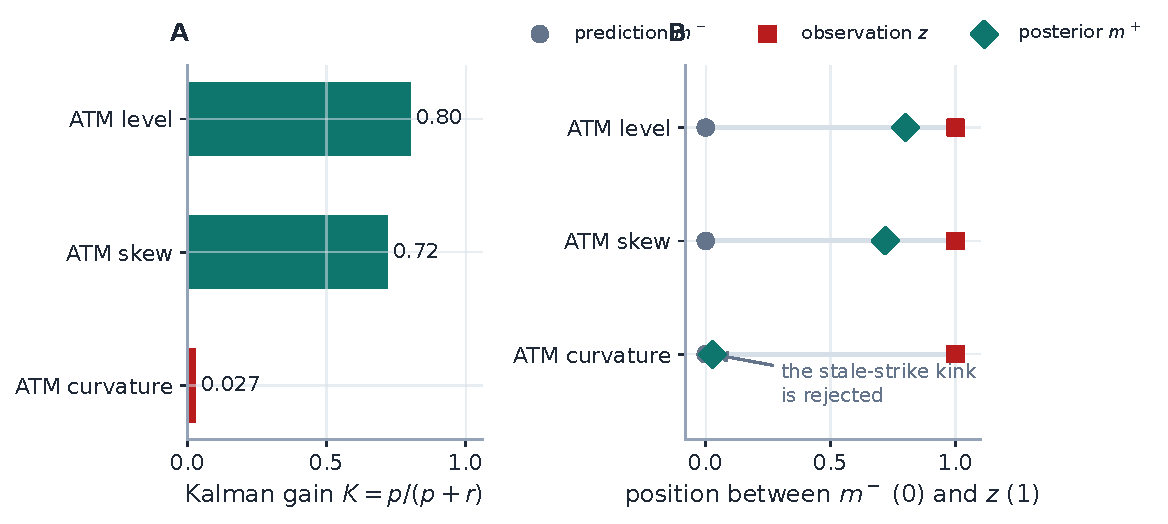
\includegraphics[width=\textwidth]{fig_kalman_case.pdf}
\caption{The case file through the production update. (A)~The tight level and
skew observations are accepted at gains \KalGainLevel\ and \KalGainSkew; the
contradiction-inflated curvature passes at \KalGainCurv. (B)~Each posterior
lands on the prediction$\to$observation segment exactly at its gain: the
level moves to the market, the stale-strike curvature kink is rejected ---
without any gap logic ever firing.}
\label{fig:case}
\end{figure}

This example is deliberately small, but it captures the implementation rule: a
dense cluster with a bad internal residual is not a gap; it is a high-$R_t$
observation. A strike range with no reliable quotes is a gap; it belongs to
prior persistence.

\begin{example}[title={Case file: the off-diagonal blow-up on coarse chains}]
\textbf{Setup.} The Phase-5 temporal backtest replayed the August 2024 spike
day pair across the eight pilot assets in overlay mode, full-covariance
update, Jacobian route --- the design configuration of \cref{eq:kalman}
verbatim.

\textbf{Failure mode.} On EEM and EFA --- coarse-strike, wide-spread ETF
chains --- the posterior ATM error reached
\KalBlowupMinPts--\KalBlowupMaxPts\ \emph{vol points}, worse than \emph{both}
baselines (the raw measurement and the gain-zero prediction). A scalar update
cannot do that: by \cref{prop:scalar} its posterior is a convex combination of
prediction and observation. The blow-up had to be a cross-handle effect.

\textbf{Diagnosis.} On a coarse chain the Jacobian covariance
\cref{eq:cov-delta} carries strong level--curvature correlations (few strikes
identify level and curvature jointly, not separately). A junk curvature
innovation --- the very thing the filter is supposed to swallow --- then drags
the ATM level through the \emph{off-diagonal} entries of
$K=P^-S^{-1}$. The pilot cap is no defence: \texttt{filterMaxGain} caps the
own-gains $\diag(KH)$ only, and the damage travels through the off-diagonal
terms it never touches.

\textbf{Fix.} Production diagonalizes $P^-$ and $R$ before the update
(\texttt{DIAGONAL\_UPDATE} in \texttt{volfit/api/observation\_filter.py}):
per-handle scalar gains, the Note~14 graph convention
(\cref{rem:diagonal}). The full-covariance update remains available for later
study --- the correlations are real information, and using them safely (e.g.\
through a correlation shrinkage) is future work, not a revert.

\textbf{Verdict.} Post-fix, EEM wins against the raw measurement
(\KalEEMPost\ vs \KalEEMMeas\ bp, $\zeta$ mean \KalEEMZeta) and EFA degrades
gracefully --- near-zero gain from its wide-spread $R$, $\zeta$ mean
\KalEFAZeta, i.e.\ conservative rather than wrong. The behaviour is locked by
\texttt{test\_observation\_filter\_app.py}.
\end{example}

%======================================================================
\section{What the backtest measured}
\label{sec:backtest}

The filter was not accepted because charts look smooth. The temporal harness
\texttt{backend/backtest/observation\_filter.py} drives the \emph{production}
commit path over consecutive captured day pairs in three market regimes
(the August 2024 spike, October 2022 high-vol, July 2023 low-vol), eight
assets each: fit day $T{-}1$'s full chain and commit it through the filter;
carry the state into day $T$ with the real snapshot-timestamp $\Delta t$ and
forward transport; build day $T$'s measurement from a \emph{thinned} ATM-only
chain under a scenario; score the posterior against the day-$T$ full-chain
truth and against \emph{two} baselines --- the raw measurement (no filter) and
the pure transported prediction (gain $0$). Three scenarios probe the three
failure modes: \texttt{thinned} (plain consecutive snapshots),
\texttt{contradiction} (two adjacent near-ATM strikes kinked in opposite
directions --- curvature noise that must be rejected), and \texttt{shock} (a
true $+5$ vol-point jump with unchanged spreads --- a move that must be
followed). Calibration of uncertainty is scored by the standardized residual
$\zeta=(\text{truth}-m^+)/\sqrt{P^++R_{\mathrm{truth}}}$ --- the truth is
itself a fitted estimate, and scoring against $\sqrt{P^+}$ alone overstated
miscalibration threefold. Results are bucketed by maturity
($\le30$ and $>30$ days to expiry). Two full sweeps were run: the
\KalStepsTotal-step \emph{tuning} sweep (overlay only) that settled the clock
noise and the covariance route, and a \KalStepsVTwo-step \emph{v2} sweep ---
overlay \emph{and} active modes, adaptive $Q$ on --- that scored the shipped
configuration end-to-end. \Cref{fig:backtest} shows the two headline panels;
the numbers below are at the decision cell (Jacobian route, thinned, $>30$d)
of the tuning sweep unless stated.

\begin{figure}[H]
\centering
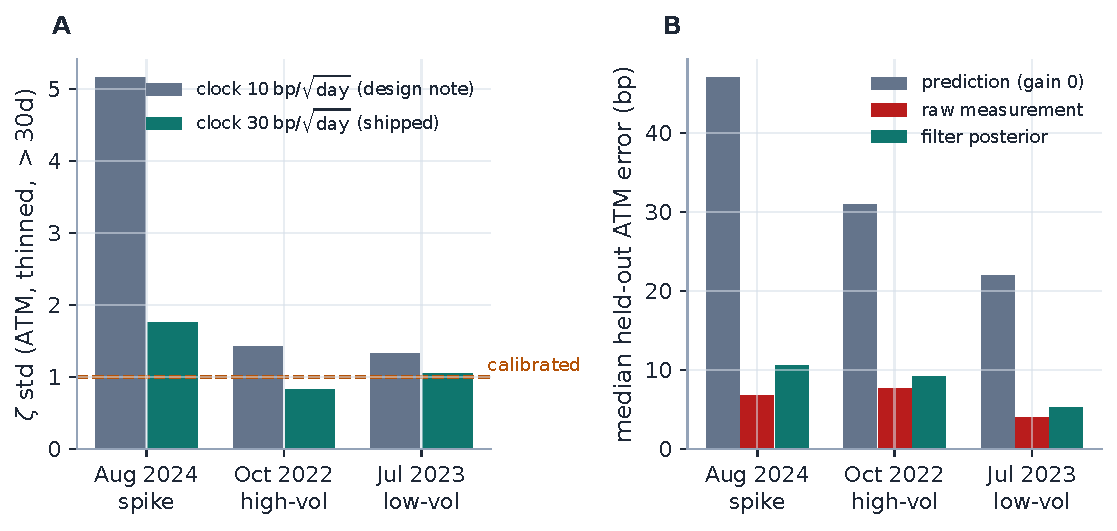
\includegraphics[width=\textwidth]{fig_kalman_backtest.pdf}
\caption{(A)~Tripling the clock noise collapses the $\zeta$ standard
deviation toward the calibration target of $1$ in every regime
(\KalZstdSpikeTen$\to$\KalZstdSpikeThirty, \KalZstdHighTen$\to$\KalZstdHighThirty,
\KalZstdLowTen$\to$\KalZstdLowThirty): the design value of
$10$ bp$/\sqrt{\text{day}}$ starved the prediction uncertainty. (B)~On plain
thinned days the posterior sits between the raw measurement and the gain-zero
prediction: the filter pays for itself on the noisy tail, not on clean liquid
days --- exactly the success criterion.}
\label{fig:backtest}
\end{figure}

\paragraph{The clock-noise default flipped ($10\to30$).} The evidence is
one-sided: in every regime, on both covariance routes, at every scenario,
$q=30$ bp$/\sqrt{\text{day}}$ improves on the design value of $10$ --- the
$\zeta$ std collapses toward $1$ (panel A), shock lag shrinks
\KalShockImproveMin--\KalShockImproveMax$\times$, and win rates rise. A
too-small clock noise starves $P^-$, so the filter over-trusts its own
prediction and both lags real moves and reports overconfident posteriors. The
shipped default is $30$.

\paragraph{Jacobian versus factors is a real trade-off; Jacobian stays the
default.} On \texttt{contradiction} --- the filter's core denoising case ---
the Jacobian route is $2$--$3\times$ better in every regime
(high-vol: \KalContraJacHigh\ vs \KalContraFacHigh\ bp; spike:
\KalContraJacSpike\ vs \KalContraFacSpike; low-vol: \KalContraJacLow\ vs
\KalContraFacLow): its geometry-aware $R$ sees which directions the kinked
cluster fails to identify. On \texttt{shock} the ranking reverses (spike:
\KalShockJacSpike\ vs \KalShockFacSpike\ bp lag) because the factor route's
blunter, smaller effective $R$ yields higher gain. Contradiction rejection is
the feature's purpose, the shock gap closes for both routes under the
adaptive-$Q$ item below, and the factor route stays one knob away.

\paragraph{The honest median-day statement.} On plain consecutive days the raw
measurement is already good (\KalErrMeasLow--\KalErrMeasHigh\ bp median ATM
error across regimes) and the filter's median win rate is
\KalWinSpike--\KalWinHigh\ --- \emph{below} one half. The posterior
(\KalErrPostSpike/\KalErrPostHigh/\KalErrPostLow\ bp per regime) beats the
gain-zero prediction (\KalErrPredSpike/\KalErrPredHigh/\KalErrPredLow\ bp)
everywhere but does not beat a clean measurement on a clean day, and it should
not: the filter pays for itself on the noisy tail --- the contradiction
columns, the illiquid names, the wide-spread chains --- which is precisely the
success criterion set before the backtest ran (``lower held-out error in noisy
snapshots'', not ``lower every RMS''). The slightly negative $\zeta$ means on
thinned days are a harness artifact worth recording: the ATM-window thinning
is mildly biased against the full-chain truth.

\paragraph{Documented limitations, and what shipped against them.} Two items
are measured, known, and deliberately not hidden. (i)~The $\le30$ DTE bucket
is a different regime: short-dated nodes carry $90$--$160$ bp thinned-vs-full
discrepancies from quote and de-Americanization noise (the Note~04/05
short-dated diagnosis, not a filter defect), the filter loses to raw there,
and the buckets are reported separately so neither regime masks the other.
\emph{Shipped:} a maturity-scaled noise floor --- the stated per-quote noise
is multiplied by $\sqrt{30\,\mathrm{DTE}/\mathrm{DTE}}$ below $30$ DTE (never
below one), matching the measured $2$--$3\times$ short-end discrepancy and
applied consistently to $R_t$, the active MAP weights and the posterior
unwhitening. (ii)~A fixed clock cannot span calm and spike regimes.
\emph{Shipped:} innovation-gated adaptive $Q$
(\texttt{filterAdaptiveSigma}, default $3$): a per-handle surprise beyond the
gate inflates $P^-$ by $(\zeta/3)^2$ (capped) so it reads as ${\sim}3\sigma$.
Measured first on the spike fixtures (SPX shock win $0.42\to1.00$ with
$\zeta$-std $3.8\to0.8$, clean days byte-identical below the gate; on the
noisy EFA chain the gate stays quiet --- its wide-spread (and
$\rho$-inflated) $R$ shrinks the standardized innovation, so junk is not
chased), then validated at full scale by the v2 sweep: the median shock
error ($>30$d) collapses from \KalShockJacSpike\ to \KalOvlShockSpike\ bp in
the spike regime, \KalShockJacHigh\ to \KalOvlShockHigh\ in high-vol and
\KalShockJacLow\ to \KalOvlShockLow\ in low-vol, with the thinned and
contradiction cells unchanged --- the gate opens on genuine shocks and stays
quiet on clean days, as designed.

\paragraph{Active mode, measured at full scale.} The v2 sweep scores the
\texttt{active} one-stage MAP itself (\texttt{--modes overlay,active}); in
that mode the committed fit IS the MAP solution, so the baseline is the
overlay run's raw-measurement column of the same sweep. The verdict is
one-sided wherever denoising is the job: on plain thinned days the active
MAP beats \emph{both} the raw fit and the overlay posterior in every regime
(\KalActThinSpike/\KalActThinHigh/\KalActThinLow\ bp against raw
\KalErrMeasSpike/\KalErrMeasHigh/\KalErrMeasLow\ per regime), and on
contradiction days it wins outright in the high- and low-vol regimes
(\KalActContraHigh\ vs \KalRawContraHigh\ bp raw; \KalActContraLow\ vs
\KalRawContraLow) while in the spike regime it still beats the post-hoc
blend (\KalActContraSpike\ vs \KalOvlContraSpike\ bp) though not the raw fit
(\KalRawContraSpike\ bp) --- all with honest uncertainty ($\zeta$ std
\KalActZetaMin--\KalActZetaMax\ over those cells). Fitting quotes and
prediction jointly beats blending them after the fact, exactly as
\cref{prop:nodouble} says it should. The measured weakness is the shock
scenario (\KalActShockSpike--\KalActShockHigh\ bp lag in the spike and
high-vol regimes): the MAP prior weight is fixed before the measurement
exists, so the innovation-gated adaptive $Q$ --- overlay-only by
construction --- cannot open for it. Extending the gate to the active path
(gating on the previous step's innovation, or a cheap ATM pre-probe) is
\emph{the} remaining item before any active-by-default discussion.

%======================================================================
\section{What is original here}
\label{sec:original}

The Kalman equations are classical \cite{Kalman1960,AndersonMoore1979}. The
Vol-Fitter-specific contribution is the separation of three notions that are
usually blended in volatility tools:
\begin{enumerate}[leftmargin=1.6em]
\item \textbf{Quote likelihood}: today's prepared quotes, with bands, weights
and no-arbitrage model structure (Note~07).
\item \textbf{Temporal filtering}: a transported latent smile state with
prediction and measurement covariance.
\item \textbf{Gap persistence}: a prior that activates only where current
quotes do not identify a functional (Note~13).
\end{enumerate}
That separation is what makes the feature safe: the filter denoises a noisy
observed smile without using yesterday as a fake quote, and prior persistence
stabilizes unobserved wings without damping a real current-market move. Two
implementation pieces are worth singling out beyond the architecture. The
\emph{measurement covariance in stated noise} (\cref{sec:units}): tying
$J\T WJ$ to the bid--ask half-spread is what makes $R_t$ a market object
rather than a fit artifact, and the same scalar $s_q$ then makes the active
MAP weights and the posterior information mutually consistent. And the
\emph{ungated stencil prior} (\cref{sec:active}): expressing $(m^-,P^-)$ as
exact ATM-stencil operator targets lets one prediction prior steer every
parametric model through existing plumbing, while the hard-coded persistence
auto-exclusion makes double-anchoring impossible rather than discouraged.

%======================================================================
\section{Limitations}
\label{sec:limits}

The diagonal update discards genuine cross-handle information by design; the
off-diagonal blow-up of \cref{sec:case} showed why that trade is currently
right, but a shrunk-correlation update is a live research item, not a closed
door. The clock process noise is a fixed scalar; the shipped
innovation-gated adaptive $Q$ (\cref{sec:backtest}) recovers genuine jumps,
but it inherits the measurement's trustworthiness --- on wide-spread
illiquid chains it deliberately stays quiet, so those names still lag real
moves --- and it is overlay-only: the active MAP's prior weight is fixed
before the measurement exists, so active mode lags genuine shocks
(\KalActShockSpike--\KalActShockHigh\ bp in the v2 sweep) until the gate is
extended to the fit path. Short-dated nodes ($\le30$ DTE) are dominated by quote and
de-Americanization noise; the shipped $\sqrt{30/\mathrm{DTE}}$ noise floor
sizes $R_t$ honestly there, but honest uncertainty is not signal --- the
short end remains the filter's weakest bucket. The state is per-node: a graph-coupled filter
(Note~14's block covariance with time dynamics) is deferred until the
single-node filter has earned trust. And the measurement carrier is the LQD
backbone: a displayed model whose handles disagree with the backbone's inherits
that disagreement through the overlay.

%======================================================================
\section{Traceability}
\label{sec:traceability}

\begingroup
\small
\setlength{\tabcolsep}{3pt}
\begin{longtable}{@{}p{0.34\textwidth}p{0.14\textwidth}p{0.24\textwidth}p{0.22\textwidth}@{}}
\caption{Claims in this note and the code/tests that lock them.}\\
\toprule Claim & Object & Code anchor & Test anchor\\ \midrule
\endfirsthead
\toprule Claim & Object & Code anchor & Test anchor\\ \midrule
\endhead
Joseph update PSD for any gain; own-gain cap; scalar shrinkage; agrees with
the graph posterior to $10^{-12}$ &
\cref{eq:kalman}, \cref{prop:scalar} &
\nolinkurl{volfit/calib/observation_filter.py} &
\nolinkurl{test_observation_filter.py}\\
One-stage MAP minimizer $=$ Kalman posterior to $10^{-10}$; ungated stencil
prior; no second update &
\cref{prop:nodouble}, \cref{eq:active-map} &
\nolinkurl{volfit/calib/observation_filter.py},
\nolinkurl{volfit/api/observation_filter.py} &
\nolinkurl{test_observation_filter.py},
\nolinkurl{test_filter_active.py}\\
Jacobian covariance; regularized eigen-inverse; stated-noise units contract &
\cref{eq:cov-delta} &
\nolinkurl{volfit/calib/observation_measurement.py} &
\nolinkurl{test_observation_measurement.py}\\
Contradictions inflate $R$; band rows contribute nothing inside the spread &
\cref{eq:resid-inflation} &
\nolinkurl{volfit/calib/observation_measurement.py} &
\nolinkurl{test_observation_measurement.py}\\
Diagonal update; idempotent commits; reset matrix; seeding without a hidden
fit &
\cref{rem:diagonal}, \cref{sec:lifecycle} &
\nolinkurl{volfit/api/observation_filter.py} &
\nolinkurl{test_observation_filter_app.py}\\
Mode resolution; \texttt{off} byte-identical; overlay never steers fits &
\cref{sec:architecture} &
\nolinkurl{volfit/api/filter_mode.py} &
\nolinkurl{test_filter_mode.py}\\
Persistence auto-exclusion: only the deep-tail anchor and dark nodes survive
in active mode &
\cref{sec:active} &
\nolinkurl{volfit/api/prior_mode.py} &
\nolinkurl{test_filter_active.py}\\
Temporal backtest protocol, scenarios and $\zeta$ scoring &
\cref{sec:backtest} &
\nolinkurl{backend/backtest/observation_filter.py} &
\nolinkurl{test_filter_backtest.py}\\
\bottomrule
\end{longtable}
\endgroup

\appendix
%======================================================================
\section{Hyperparameter atlas}
\label{app:atlas}

Every knob touching the observation filter, with its shipped default and role.
Surfaced knobs are user-facing \texttt{OptionsSettings}; hidden knobs are
internal constants tuned to the algorithm.

\begingroup
\small
\begin{longtable}{p{0.34\textwidth}p{0.13\textwidth}p{0.45\textwidth}}
\caption{Observation-filter hyperparameters, as shipped.}\label{tab:atlas}\\
\toprule Knob & Default & Role\\ \midrule
\endfirsthead \toprule Knob & Default & Role\\ \midrule \endhead
\multicolumn{3}{l}{\emph{Surfaced (OptionsSettings)}}\\ \midrule
\texttt{observationFilterMode} & \texttt{off} &
\texttt{off} / \texttt{overlay} / \texttt{active}
(\cref{sec:architecture}); \texttt{off} is byte-identical to the feature
never existing.\\
\texttt{filterCovarianceMode} & \texttt{jacobian} & Measurement-covariance
route: \texttt{jacobian} \cref{eq:cov-delta} (backtested default,
\cref{sec:backtest}) or \texttt{factors} \cref{eq:cheapR} (fallback + A/B
column).\\
\texttt{filterProcessVolBpSqrtDay} & $30$ & ATM clock process noise in vol bp
per $\sqrt{\text{day}}$. Backtested: the design value $10$ starved $P^-$ in
every regime; $30$ is one-sided better (\cref{fig:backtest}A).\\
\texttt{filterProcessSkewSqrtDay} & $0.02$ & Skew clock process-noise scale.\\
\texttt{filterProcessCurvSqrtDay} & $0.05$ & Curvature clock process-noise
scale.\\
\texttt{filterTransportNoiseScale} & $0.10$ & Extra process std per unit
$\abs{\log(F_t/F_{t-1})}$ transport distance (\cref{eq:Q} spot term).\\
\texttt{filterResidualInflation} & on & Apply \cref{eq:resid-inflation} so a
dense-but-contradictory cluster reads as measurement noise.\\
\texttt{filterAdaptiveSigma} & $3$ & Innovation-gated adaptive $Q$
(\cref{sec:backtest}): a per-handle surprise beyond this many standardized
sigmas inflates $P^-$ by $(\zeta/\text{gate})^2$, capped; $0$ = off. Overlay
path only (the active MAP prior precedes the measurement).\\
\texttt{filterMaxGain} & $1.0$ & Pilot safety cap on the per-handle own-gains;
at $1.0$ it never binds (own-gains sit in $(0,1)$ by construction).\\
\texttt{filterResetHours} & $96$ & Maximum data gap the filter predicts
across; longer gaps reset as \texttt{stale} (the default spans a weekend plus
a holiday).\\
\texttt{filterDataOnlyPrepass} & off & Opt-in extra data-only fit so $z_t$ is
strictly persistence-free; off reuses the committed fit and flags
contamination instead.\\
\midrule
\multicolumn{3}{l}{\emph{Hidden (internal constants)}}\\ \midrule
\texttt{DIAGONAL\_UPDATE} & on & Per-handle scalar gains
(\cref{rem:diagonal}); the measured answer to the off-diagonal blow-up case
file.\\
\texttt{FILTER\_STENCIL\_H} & $0.06$ & ATM stencil half-width of the active
MAP prior legs; the stencil identities are exact on a locally quadratic
smile.\\
\texttt{RESID\_INFLATION\_CAP} & $25$ & Cap on $\rho_t$ in
\cref{eq:resid-inflation}: one broken chain cannot poison the state. Also
caps the adaptive-$Q$ inflation factors.\\
\texttt{SHORT\_DATED\_REF\_DAYS} & $30$ & Short-dated noise floor: the stated
per-quote noise is scaled by $\sqrt{30/\mathrm{DTE}}$ below $30$ DTE (never
below one), consistently in $R_t$, the active MAP weights and the posterior
unwhitening.\\
\texttt{INFO\_RANK\_RTOL} & $10^{-10}$ & Relative eigenvalue cutoff of
$\calI_\theta$; small eigenvalues are clamped \emph{up}, so unidentified
directions inflate $R$ finitely instead of exploding or vanishing.\\
\texttt{CHOL\_JITTER} & $10^{-12}$ & Base jitter of the whitening Cholesky;
any nonzero use is reported as a diagnostic event, never silent.\\
\texttt{HANDLE\_MOVE\_SCALES} & $(0.03,0.05,0.5)$ & Typical one-day move
scales giving the dimensionless transport knob a per-handle magnitude (the
Note~14 units convention).\\
\texttt{RMS\_FLOOR} & $10^{-4}$ & Floor on the stated per-quote noise (one vol
bp): an excellent fit is not infinitely precise. Chains without band data use
$10\times$ this floor.\\
variance envelope & graph floors/caps & Per-handle $R$ diagonals are clipped
into $[1/\text{cap},1/\text{floor}]$ from
\nolinkurl{volfit/graph/precision.py}, correlations rescaled to survive.\\
\texttt{\_filter\_version} & --- & Overlay-only knob changes bump a
lightweight version so the overlay refreshes without invalidating any fit
cache; only \texttt{active}-affecting changes bump the options version.\\
\bottomrule
\end{longtable}
\endgroup

%======================================================================
\section{Performance notes}
\label{app:perf}

\begin{enumerate}[leftmargin=1.6em]
\item \textbf{Overlay mode is invisible next to calibration.} The update is a
dense $d\times d$ solve with $d=3$; state storage is $O(d^2)$ per node.
\item \textbf{The Jacobian covariance is nearly free.} $J\T WJ$ comes from the
solution Jacobian the calibrators already retain, and the handle Jacobian $G$
is $2P$ slice \emph{builds} (no fitting) on the coarse optimization grid ---
about $4\times$ cheaper per build than the display quadrature.
\item \textbf{Seeding must never hide a fit.} The first implementation seeded
through the prior bootstrap branch, whose fetch path silently ran a \emph{full
extra mid calibration per node}; switching the filter on made a live universe
crawl. The shipped rule: seed from the transported saved prior when one
exists, else from the committed fit's own handles at bootstrap-tier precision
--- the same information, for free. Reverted-and-redesigned, per house
practice.
\item \textbf{Overlay curves are memoized per committed state.} The filtered
curve is the backbone retargeted to $m^+$ (a Newton solve, Note~01); computing
it per GET made the live UI feel frozen, since the smile view polls the
payload on every refresh signal. It is now computed once per committed state.
\item \textbf{Active MAP adds no second fit pass.} The prediction prior is
three residual rows in the existing least-squares stack; the optional
data-only prepass is the only real cost lever and is off by default.
\item \textbf{Graph generalization is natural but later.} A graph Kalman
filter replaces the per-node $P_t^-$ with a block covariance over the universe
--- Note~14's covariance-form posterior with time dynamics. It comes after the
single-node filter has earned trust.
\end{enumerate}

%======================================================================
\section{Reference implementation}
\label{app:ref}

The numerical heart is small and model-free: it assumes the caller has already
built the prediction and measurement moments. The listing below is executed by
\texttt{gen\_kalman.py} against the production
\texttt{volfit.calib.observation\_filter.kalman\_update} on a random-seeded
$3\times3$ problem (full covariances, $H=I$); the maximum deviation across
mean, covariance, innovation, innovation covariance and gain is
$\KalRefAgreement$ --- machine precision, as it should be, since production
adds only input validation, the own-gain cap and the PSD guard around the same
algebra.

\begin{lstlisting}[caption={Covariance-form Kalman update with Joseph
covariance (verified against production; agreement stated above).}]
def kalman_update_ref(mean_pred, cov_pred, obs, obs_cov, H=None):
    m = np.asarray(mean_pred, dtype=float)
    P = np.asarray(cov_pred, dtype=float)
    z = np.asarray(obs, dtype=float)
    R = np.asarray(obs_cov, dtype=float)
    H = np.eye(m.size) if H is None else np.asarray(H, dtype=float)
    innovation = z - H @ m
    S = H @ P @ H.T + R
    K = np.linalg.solve(S.T, (P @ H.T).T).T
    out_mean = m + K @ innovation
    I_KH = np.eye(m.size) - K @ H
    out_cov = I_KH @ P @ I_KH.T + K @ R @ K.T
    return out_mean, 0.5 * (out_cov + out_cov.T), innovation, S, K
\end{lstlisting}

The active-mode residual rows corresponding to \cref{eq:active-map} are
equally small once the model exposes a handle extractor:

\begin{lstlisting}[caption={Whitened residual rows for the active MAP
prediction prior (distilled from
\texttt{volfit/calib/observation\_filter.py}).}]
def prediction_prior_residual(model_handles, mean_pred, cov_pred):
    L = np.linalg.cholesky(np.asarray(cov_pred, dtype=float))
    return np.linalg.solve(L, np.asarray(model_handles) - np.asarray(mean_pred))
\end{lstlisting}

In production the Cholesky solve uses a small escalating jitter and reports
it; adding jitter is a diagnostic event, not a silent repair.

\begin{thebibliography}{9}
\bibitem{Kalman1960} R.~E.~Kalman. A new approach to linear filtering and
prediction problems. \emph{Journal of Basic Engineering}, 82(1):35--45, 1960.
\bibitem{AndersonMoore1979} B.~D.~O.~Anderson and J.~B.~Moore.
\emph{Optimal Filtering}. Prentice-Hall, 1979.
\bibitem{Gelman2013} A.~Gelman et al. \emph{Bayesian Data Analysis}. CRC
Press, 3rd ed., 2013.
\bibitem{Gatheral2006} J.~Gatheral. \emph{The Volatility Surface}. Wiley,
2006.
\end{thebibliography}

\end{document}
